\section{Qualitative Civilization}

\begin{wrapfigure}{rt}{.3\textwidth}
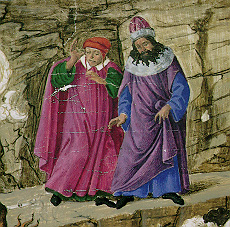
\includegraphics[width=.3\textwidth]{botticelliDanteVirgil.jpg}
\end{wrapfigure}

\begin{quotex}
True progress will always respect the line of formal development of man. It will give rise to \emph{qualitative} civilization such as was the civilization of Greece in the fourth century BC and, in a higher degree, the civilization of Western Europe in the thirteenth century. If a people's attention is diverted from things spiritual and turned to material conquests, to the cultivation of the useful, that is, of whatever serves as a means of furthering human intercourse and ministers to man's bodily needs and comforts, the whole direction of life gradually changes. The means become the end. The civilization is \emph{quantitative} instead of \emph{qualitative}.
\flright{\textsc{Denis Fahey CSSp}, \emph{The Mystical Body of Christ in the Modern World}, p 140}
\end{quotex}


In this passage, we see the fundamental agreement between Fr. Fahey (a Traditional Catholic), \textbf{Rene Guenon}, and \textbf{Julius Evola}, all of whom see the last of a Traditional civilization in the civilization of Western Europe in the thirteenth century. Therefore, it is worth investigating in more detail the characteristics of that civilization that make it so. It often seems easier to look further beyond, say to India, or pagan Scandinavia, and so on, although this is prone to many misconceptions and misunderstandings. On the other hand, something closer is often more emotionally challenging, particularly is we are accustomed to look at the period as the ``Dark Ages'' marked by theocratic or feudal oppression. Yet, if we take Guenon and Evola seriously, then we must take this period seriously, and it must be done objectively without prejudices or \emph{a priori} commitments to particular theological positions.

To be clear, we stand with Maurras\footnote{\url{https://www.gornahoor.net/?p=453\#WesternCiv}} and take the West as a single civilization: ``The Western Tradition is based on the axis from Greece and Rome, and its prolongation in time to Paris''. This is unlike Evola, who saw two distinct civilizations. Also, unlike Guenon, we see that Tradition as complete and not inferior to anything East of Persia. This is called the Roman Tradition, or Romanity.

The method used will be to look at the natural order in the development of truly human life within a civilization. This encompasses several fields of human endeavour.

\begin{itemize}


\item Metaphysics

\item Art

\item Science

\item Politics

\item Economics and Technics

\item Ethics and Civic Virtues
\end{itemize}


The profane historian interests himself in the contingent realm of politics or economics. Thus, he calls the ``Fall of Rome,'' what was in reality a regime change. The alternative is to see in the Germanic tribes nothing but barbarian hordes and in Rome just a political structure while missing its essential Spirit. Rather, we see that era as the incorporation of the Germanic and Nordic Traditions into Romanity; the incursions of the Northern peoples---who saw themselves as Roman---into Southern Europe brought political and economic disruption, but then led to the enrichment of Romanity and its continuation under a different form. The actual \textbf{Fall of Rome}, in the metaphysical sense, came much later.

We shall briefly mention two representative figures of thirteenth century Europe to demonstrate the continuity of the Roman Tradition. They represent the fields of metaphysics and art.

\paragraph{Thomas Aquinas}


Thomas Aquinas connects ancient Athens to medieval Paris by incorporating the philosophy of Aristotle, Plato, and indirectly Plotinus through Dionysus and Augustine. His metaphysical doctrine, known now as Thomism, was regarded by both Guenon and Evola to embody Tradition.

\paragraph{Dante Alighieri}


The great poet Dante looked to the Roman poet Virgil\footnote{\url{http://users.erols.com/antos/dante/why\_virg.html}} as his guide, which indirectly connects him to to \textbf{Homer}. Evola, Guenon, and Coomaraswamy---who considered Dante to be one of the greatest of Europeans\footnote{\url{https://www.gornahoor.net/?p=556}}---held Dante in high esteem from a Traditional perspective. Furthermore, through his relationship to the \emph{Fedeli d'Amore}, Dante can be regarded as an initiate, demonstrating the existence in the West of an authentic esoteric tradition.


\flrightit{Posted on 2011-01-02 by Cologero}

\begin{center}* * *\end{center}

\begin{footnotesize}
\begin{sffamily}
\texttt{James O'Meara on 2011-01-03 at 19:13 said:}

Cologero,

A worthy project, but two questions, conveniently keyed to our Traditionalist spokesmen:

Evola and Two Tradtions; you mean, ``pagan'' and Christian, not Greek and Roman, yes? If so, how do you account for the way Christians, from Justin A. to the vulgar radio preacher, delight in pointing out just that, that Christianity is a different tradition? Either they mock the pagans as stupid or demon-deceived, or else they are glad to take over the pagan and ``improve'' it just a little hear and there. Just this morning, a radio preacher gave me the first; then, on the subway, reading a book of Anglo Saxon translations, the editor gave me the ``how the poems show Christian ideas entering and gradually proving superior to the authors' native paganism'' line. And you've already discussed Ph. Sherrard gently moving Anthony to the appendix of the Philokalia trans. Even Dante could do no more with the pagans than stick them in a comfy waiting room like the one in Beetlejuice . He clearly sees them as worthy but different, thus needing a different treatment. Well, except for Cassius and Brutus... And Guenon; he locates the `superiority' of Eastern metaphysics in general he clearly makes exceptions for occasional Westerners with superior knowledge in a curious inability of Westerners to form non-concrete or non-utilitarian ideas. One example is the inability although proudly flaunted, in accordance with question one to conceive of a metaphysical principle beyond being and non-being, consequently locating supreme reality in Being. This is the essence of the superiority of metaphysics to mere religion. His remarks on this in Reign of Quantity, for example, certainly jibe with what I was being taught at the time I was reading him, years ago, in a small ex-Catholic college now staffed by PhDs from the Pontifical Institute who had gone through not only Gilson but Jos. Owens' dogmatic views on ``the Doctrine of Being'' in Aristotle and Thomas. Again, nothing was higher than Being, that's just it, take it or leave it. Again, you can find ``mystics'' saying otherwise, but they're treated as heretics or else, among philosophers, dismissed as Hegel another Being guy does Schelling, ``lost in the dark night where all cows are black.''

\hfill

\texttt{Cologero on 2011-01-03 at 22:33 said:}

James, why then do your favorite radio preachers consider the tradition 13th century Europe to be pagan? Maybe in spite of themselves, they see something you don't. This post needs to be understood in the light of what we have posted before in preparation; of course, more will follow. First of all, we are aiming at specificity; the post did not mention ``Christianity'' at all, referring instead to a particular period of time, mainly to avoid the projections and prejudices you display.

We can only make the following points at this time:

1) It's curious that Guenon attributes a racial cause to some alleged inability of ``Westerners''. Perhaps, then, Easterners have their own racial defect. Perhaps they fail to see the relationship between ideas and the world process and the question of the Will. That is dealt with in the Tantras, or the ``Fifth Veda'', which Guenon concedes may be appropriate for the Kali Yuga. Since G. sticks to the orthodox schools of Hinduism, he may have inadvertently left something out.

2) For Aquinas, God is the principle of being, though an Eckhart can understand the God beyond God, that is, God as Absolute and Infinite, beyond Being. G. tried to awaken Maritain to that. Oddly enough, in the 1933 lectures on Being (long after G had left town), Maritain mentions Shankara, Aristotle, and Aquinas in the same breath. That is an idea that needs to be developed. Also, 20th century neo-Thomists are not Thomists; they purge the Platonic elements and fail to understand the intellect as a form of knowledge. In the Hindu Doctrines, G accepts the Platonic tradition as having a fuller understanding.

3) We have mentioned many thinkers from the ancients to a Soloviev who see a connection to ancient Egypt. Even a Catholic Bishop could write this as late as 1865: ``We neither derive our religion from the Scriptures, nor does it depend upon them. Our faith was in the world before the New Testament was written.'' (Cardinal Manning)

4) The conflict between ``mystics'' and theologians will be dealt with at a later time. Suffice it to say, for now, that mystics, gnostics, or Hermetists may also play a part in ``Tradition'', even if not necessarily part of the visible theological tradition.

Is there work to be done? Obviously, because of the actual Fall of Western Tradition, we are at this time bloodhounds sniffing out the trail. Rest assured that your radio preacher knows nothing of Tradition; we also cannot recommend worshiping at the feet of some Asian guru. We see nothing superior in that.

\hfill

\texttt{kadambari on 2011-01-04 at 10:38 said:}

Well for us, disruption of civilization, that is, tradition, occurs with the arrival of Islam. British colonialism is just a consequence of that as centuries of Islam had weakened and impoverished India. Also I think Buddhism after losing conncetion to Indian aristocracy after the fall of the North West (Afghanistan, Pakistan) offers little that is of interest. Almost all of the worthwhile Sutras are written by Indians, with the exception of a few written by Chinese monks. Systems like Zen resemble more vodoo to me when I read it and even that was founded by Bodhidharma an Indian monk. This is not to say that countries like Japan do not have well organized societies and high standards of living and are impressive in that. But I do not think these societies can make Buddhism the impressive thing it was in the past, and their Buddhism is merely local, there are no impressive Buddhist teachers anymore who can command global interest and respect.

If India can get past the menace of Islam at all levels and minimize the influence of Abrahamic thinking on the culture, if it provide for a better standard of living for its people, I think this can lead to religious renewal there... \hfill

\texttt{kadambari on 2011-01-04 at 11:17 said:}

``Thus, he calls the ``Fall of Rome,'' what was in reality a regime change. The alternative is to see in the Germanic tribes nothing but barbarian hordes and in Rome just a political structure while missing its essential Spirit. Rather, we see that era as the incorporation of the Germanic and Nordic Traditions into Romanity; the incursions of the Northern peoples---who saw themselves as Roman---into Southern Europe brought political and economic disruption, but then led to the enrichment of Romanity and its continuation under a different form. The actual Fall of Rome, in the metaphysical sense, came much later.''

Brabarian people increase the vigor of civilization if they are absorbed by civilization by bringing in young blood and vigor. Look at the Scythian waves in India, it only added to the vigor as it assimilated into the native civilization, assimilation and a preservation of the civilizational ideals and ethos is key. Later on in Rome, many of the Senators came from provinces, so there is an assimilating effect... I hope the Western world recovers its ``Romanity'' as you put it, as the genius of the West is in Greece and Rome... 

\hfill

\texttt{Will on 2011-01-04 at 12:26 said:}

James, I don't think Dante's view of pagans and pagan traditions is as simple as you portray it. The person who guides souls through the early stages of Purgatory is Cato, who not only was a pagan (Stoic) but committed suicide. There are other non-Christians who he places higher than First Circle waiting room. He gets around this technicality by implying that when Jesus descended to hell after the crucifixion, he saved his favorites, which included more than pious Jews like Moses.

Also, consider that Dante's three absolute worst of the worst are Judas, Brutus, and Cassius. By equating these three, he is implying an equation of Caesar and Christ, or at least the Emperor and Christ. This stems from his view, developed in the Monarchia, that Empire is the natural reflection and complement of monotheism -- one God in Heaven, one Emperor on earth. Though he was an early supporter of the Guelphs, the Commedia shows strong Ghibelline tendencies.

When I first read the Commedia, my first impression was that Dante was a pagan trying to fit into Christianity -- square peg in a round hole. But I now think that he saw Christianity as the completion and perfection of the whole Graeco-Roman tradition, and also as the unifier of this one tradition. Unfortunately, he's such a damned brilliant poet that he's mostly ignored as a philosopher, mystic, and theologian.

Has anyone read the book Lost Christianity by Jacob Needleman? It asks many of these same questions about Tradition and Christianity (though without using that language) and also contains a fascinating excerpt from the writings of a 20th century Christian mystic whom the author met on his travels.

\hfill

\texttt{James O'Meara on 2011-01-04 at 18:45 said:}

Will,

Thanks for the additional detail; I did indeed forget about Cato, and the implicit equation of Christ and Caesar. I may just be not expressing myself well, however if Dante sees ``Christianity as the completion and perfection of the whole Graeco-Roman tradition, and also as the unifier of this one tradition'' then that's exactly what I mean by the damning with faint praise alternative to total rejection. I suppose that is `one tradition' of a sort, but kinda the way Christians think the Judaic religion and scriptures are ``part of our tradition and its completion;'' Jews think otherwise, and the Talmud has it's own Dantean punishments for the false Messiah Jehoshua.

I read Needleman's book when it first came out and was quite impressed by it. I've come to think N. is a bit of a `popularizer' in the bad sense; he reminds me of what a Hegelian teacher said to us about Kaufmann's facing page commentary to the Phenomenology: seldom wrong but never profound. He's gone from one thing to another over the years,and it always seems to be something to cloak a secret Gurdjieffianism, which is something I detest secrecy, not G. necessarily . I think his most lasting contribution was back at the start, when he was pretending to be an academic philosopher; an article in Rev. of Metaphysics called ``Why Philosophy is Easy'' because, ever since the Enlightenment, it's based on ordinary experience, not initiation; very like Evola's account of initiatory knowledge in Magic . That and some of the early books are contribution enough!

\hfill

\texttt{Will on 2011-01-04 at 21:44 said:}

James, Your points are well made. I do understand that Jews and pagans alike would have a problem with their lesser positions in Dante's unified tradition. But such is hierarchy; they fared better than Mohammed and Muslims, in any case (except for Averroes, who got bonus points for his work on Aristotle.)

From a Nietzschean perspective, the reason that Christ and Christians are on the top of the hierarchy is because they had the most power when it was created. On the other hand, Muslims and Jews both have their own view of things, giving some credit to Jesus as a prophet, but not placing him at the top. Had Muslims conquered Europe during the Crusades (or if they do so demographically in the next hundred years) a different hierarchy would be put into effect. But that is slightly off-topic.

If, as Cologero states, we are bloodhounds sniffing out the trail of our lost Tradition, it seems to me that Dante is a good place to start, not least of all because so many different strands of thought come together in the Commedia, with all its history, philosophy, politics, theology, and religion. What one finds in Dante, that is lacking in most other authors, is an articulated vision of what the West is, both spiritually and politically. I do realize that this vision being more Christian than pagan is upsetting or unacceptable to some, but I'm not aware of any other vision of the West that is as complete as his.

And I agree with your assessment of Needleman. What I was most impressed with in Lost Christianity were the excerpts from the writings of the monk that he met, whose name escapes me just now.

\hfill

\texttt{Cologero on 2011-01-05 at 01:03 said:}

The relationship between the predecessor and successor is asymmetric because the owl of Minerva flies at dusk; only by looking back can we discern what happened. Guido de Giorgio rightfully points to Aeneas and Christ as the founders of the respective Roman traditions. They both come from the east, are of semi-divine origin, and ascended into Heaven as Gods. Virgil comes into play as the link, since he wrote the epic poem about Aeneas; he also wrote an enigmatic passage (in Bucolics IV) that early Christians (including Dante) interpreted as foretelling the coming of Christ.

The symbol of Rome is the Janus, looking East and West: ``Rome is the East of the West''. De Giorgio regards the fascia and the cross as the respective symbols, the cross, of course, in the sense of Guenon's book on that symbol.

\hfill

\texttt{James O'Meara on 2011-01-05 at 10:16 said:}

Stumbled across this yesterday, thought it might be interesting in this context. Regarding the French collaborationist Pierre Drieu La Rochelle:

``Drieu admired Catholicism as ``a system of complex thought'' and a religion that ``represented for European civilization the arc of its covenant'' --- the travel chest ``packed with the treasures of its experience and wisdom.''

But if he venerated Christianity sub specie æternitatis, he detested what it had become --- a religion devoid of substance, a museum relic, representing nothing more than a languishing sect, symptomatic of the general decline of the West --- just another bourgeois institution linked to Big Capital.

To this degenerate Christianity, Drieu opposed the virile Christianity of the Middle Ages, the Christianity of the Gothic cathedrals, the Christianity of the white, virile God'' --- this Christian God who ceded nothing in virility and health to the Olympian and Germanic gods.

For Drieu there was no real antagonism between Christianity and paganism, only different ways of interpreting Nature. In his eyes, orthodox Catholicism had best conserved the pagan heritage.

But beyond paganism and Christianity, Drieu believed there existed a sort of universal syncretism --- a ``secret, profound religion linking all religions expressive of Man'' --- unique, yet everywhere the same.''

\hfill

\texttt{Cologero on 2011-01-05 at 13:24 said:}

Drieu was a complex man, apparently ... hard thinking and hard living, often in contradiction. He wrote:

\begin{quote}
\footnotesize
It is a type of man who rejects culture, whose resolve is stiffened in the midst of his sexual and alcoholic depravity and dreams of giving the world a physical discipline with radical effects. It is a man who does not believe in ideas, and hence rejects doctrines. It is a man who only believes in acts and carries out these acts in line with a nebulous myth
... 
\end{quote}


Yet he was a womanizing artist, of great culture, who dreamed of being a monk ... \textbf{Narcissus and Goldmund} in a single body.

On the question of ``style'', compare to Nietzsche: \textit{One thing is needful}\footnote{\url{http://www.gornahoor.net/Hyperborean.htm\#needful}}.

\hfill

\texttt{Mark on 2011-01-05 at 21:15 said:}

There is an interesting criticism about Medieval philosophy from Pierre Hadot. It is not the standard criticism that they lack the epistemological precision of Modern Philosophy (revelation having epistemological priority over sense experience or reason), but one that criticizes it from ``What is Ancient Philosophy'', which is the title of the book.

In, What is Ancient Philosophy, by Pierre Hadot he has these two positions, that ancient philosophy is primarily a way of life that originates in an existential choice. The discourse was there to express this way of life, but not become the essence of philosophy. Philosophy was primarily purificatory, it purified the will and intellect to reach the Nous.

Medieval philosophy made the discourse the essential aspect of philosophy, the ``ascesis'' element was eliminated, it became a way to rationally articulate the faith.

To quote a review from

\url{http://ndpr.nd.edu/review.cfm?id=1376}


``The final part of the book (``Interruption and Continuity: The Middle Ages and Modern Times'') may be summarized more briefly. Hadot credits the rise of Christianity with the decline of philosophy practiced as a way of life. Christianity positioned itself as a ``philosophy'' (in Hadot's sense) with its own regimen of spiritual exercises and spiritual goals, and as this religion came to eclipse the various pagan philosophies, it usurped their spiritual function. Eventually Christian interest in pagan philosophy was limited to its discourse, which was pressed into service as the ``handmaiden to theology,'' even as its spiritual practices were absorbed into, and substantially altered, Christian spirituality. The prevailing modern view of limiting philosophy to philosophical discourse is rooted in this usurpation. Despite several ``recurrences'' of the ancient concept of philosophy in post-Medieval times (discernible, for example, in Montaigne and even in Descartes as well as in Kant's concept of ``cosmic philosophy'') the ancient ideal is now all but lost. The book concludes with a more expansive discussion of what it means to live a philosophical life and a plea for a return to that ancient ideal (p. 275--281).''


\hfill

\end{sffamily}
\end{footnotesize}

